\centering
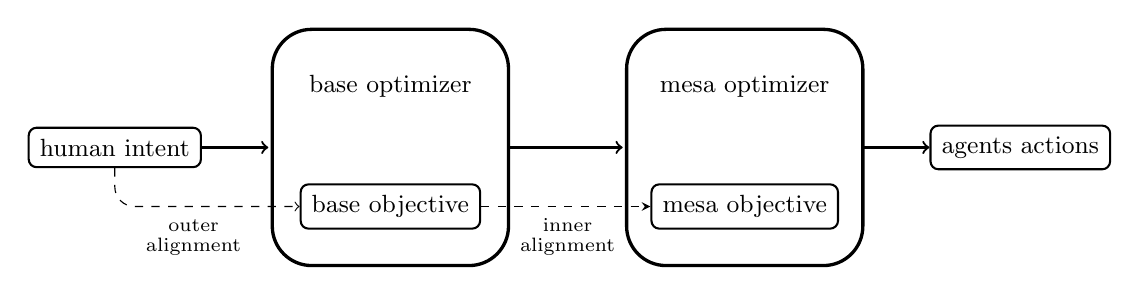
\begin{tikzpicture}[
  % GLOBAL CFG
  font=\scriptsize,
  % Styles
  cell/.style={% For the main box
      rectangle, 
      rounded corners=5mm, 
      draw,
      very thick,
      },
  operator/.style={%For operators like +  and  x
      circle,
      draw,
      inner sep=-0.5pt,
      minimum height =.4cm,
      },
  function/.style={%For functions
      ellipse,
      draw,
      inner sep=1pt
      },
  ct/.style={% For external inputs and outputs
      rectangle, 
      rounded corners=1mm, 
      draw,
      line width = .75pt,
      minimum width=1cm,
      inner sep=4pt,
      },
  gt/.style={% For internal inputs
      rectangle,
      draw,
      minimum width=10mm,
      minimum height=6mm,
      inner sep=1pt
      },
  empty/.style={% Empty nodes for joining arrows
      rectangle,
      draw,
      minimum width=0mm,
      minimum height=0mm,
      inner sep=0pt
      },
  mylabel/.style={% something new that I have learned
      font=\scriptsize\sffamily
      },
  ArrowC1/.style={% Arrows with rounded corners
      rounded corners=.25cm,
      thick,
      },
  ArrowC2/.style={% Arrows with big rounded corners
      rounded corners=.5cm,
      thick,
      },
  ]
    
    %Start drawing the thing...    

  % Draw the cell: 
  \node [cell, minimum height =3cm, minimum width=3cm] at (0,0){} ;
  \node [cell, minimum height =3cm, minimum width=3cm] at (4.5,0){} ;

  \node [empty, label={\small base optimizer}] (name1) at (0, 0.5) {};
  \node [empty, label={\small mesa optimizer}] (name2) at (4.5, 0.5) {};
  \node [empty, label={outer}] (name2) at (-2.5, -1.2) {};
  \node [empty, label={alignment}] (name2) at (-2.5, -1.5) {};
  \node [empty, label={inner}] (name2) at (2.25, -1.2) {};
  \node [empty, label={alignment}] (name2) at (2.25, -1.5) {};

  \node [ct] (human) at (-3.5, 0) {\small human intent};
  \node [ct] (acts) at (8, 0) {\small agents actions};

  \node [ct, minimum width=2cm] (optim1) at (0,-0.75) {\small base objective}; 
  \node [ct, minimum width=2cm] (optim2) at (4.5,-0.75) {\small mesa objective}; 
  
  \draw [dashed,->,style={rounded corners=.25cm}] (human) |- (optim1);
  \draw [dashed,->] (optim1) [-stealth] -- (optim2);

  \draw [->, thick] (human) -- (-1.55,0);
  \draw [->, thick] (1.5, 0) -- (2.95,0);
  \draw [->, thick] (6, 0) -- (acts);

\end{tikzpicture}
